\PassOptionsToPackage{unicode=true}{hyperref} % options for packages loaded elsewhere
\PassOptionsToPackage{hyphens}{url}
%
\documentclass[12pt,]{article}
\usepackage{lmodern}
\usepackage{amssymb,amsmath}
\usepackage{ifxetex,ifluatex}
\usepackage{fixltx2e} % provides \textsubscript
\ifnum 0\ifxetex 1\fi\ifluatex 1\fi=0 % if pdftex
  \usepackage[T1]{fontenc}
  \usepackage[utf8]{inputenc}
  \usepackage{textcomp} % provides euro and other symbols
\else % if luatex or xelatex
  \usepackage{unicode-math}
  \defaultfontfeatures{Ligatures=TeX,Scale=MatchLowercase}
    \setmainfont[]{Times New Roman}
\fi
% use upquote if available, for straight quotes in verbatim environments
\IfFileExists{upquote.sty}{\usepackage{upquote}}{}
% use microtype if available
\IfFileExists{microtype.sty}{%
\usepackage[]{microtype}
\UseMicrotypeSet[protrusion]{basicmath} % disable protrusion for tt fonts
}{}
\IfFileExists{parskip.sty}{%
\usepackage{parskip}
}{% else
\setlength{\parindent}{0pt}
\setlength{\parskip}{6pt plus 2pt minus 1pt}
}
\usepackage{hyperref}
\hypersetup{
            pdftitle={Analyzing Fecal Coliform Concentrations within Surface Waters of North Carolina},
            pdfauthor={Masha Edmondson},
            pdfborder={0 0 0},
            breaklinks=true}
\urlstyle{same}  % don't use monospace font for urls
\usepackage[margin=2.54cm]{geometry}
\usepackage{graphicx,grffile}
\makeatletter
\def\maxwidth{\ifdim\Gin@nat@width>\linewidth\linewidth\else\Gin@nat@width\fi}
\def\maxheight{\ifdim\Gin@nat@height>\textheight\textheight\else\Gin@nat@height\fi}
\makeatother
% Scale images if necessary, so that they will not overflow the page
% margins by default, and it is still possible to overwrite the defaults
% using explicit options in \includegraphics[width, height, ...]{}
\setkeys{Gin}{width=\maxwidth,height=\maxheight,keepaspectratio}
\setlength{\emergencystretch}{3em}  % prevent overfull lines
\providecommand{\tightlist}{%
  \setlength{\itemsep}{0pt}\setlength{\parskip}{0pt}}
\setcounter{secnumdepth}{5}
% Redefines (sub)paragraphs to behave more like sections
\ifx\paragraph\undefined\else
\let\oldparagraph\paragraph
\renewcommand{\paragraph}[1]{\oldparagraph{#1}\mbox{}}
\fi
\ifx\subparagraph\undefined\else
\let\oldsubparagraph\subparagraph
\renewcommand{\subparagraph}[1]{\oldsubparagraph{#1}\mbox{}}
\fi

% set default figure placement to htbp
\makeatletter
\def\fps@figure{htbp}
\makeatother

\usepackage{etoolbox}
\makeatletter
\providecommand{\subtitle}[1]{% add subtitle to \maketitle
  \apptocmd{\@title}{\par {\large #1 \par}}{}{}
}
\makeatother

\title{Analyzing Fecal Coliform Concentrations within Surface Waters of North
Carolina}
\providecommand{\subtitle}[1]{}
\subtitle{\url{https://github.com/m12edmon/FinalProject.git}}
\author{Masha Edmondson}
\date{}

\begin{document}
\maketitle

\newpage
\tableofcontents 
\newpage
\listoftables 
\newpage
\listoffigures 
\newpage

\hypertarget{rationale-and-research-questions}{%
\subsubsection{1. Rationale and Research
Questions}\label{rationale-and-research-questions}}

North Carolina is a national leader in livestock production, and is the
nation's second leading producer of hogs. The vast majority of livestock
are grown on concentrated animal feeding operations (``CAFOs'') designed
to maximize production efficiency by raising as many animals as
possible, as quickly as possible. Though CAFOs have resulted in massive
expansion and record profits in the livestock industry, they present
significant waste management challenges. CAFOs have been demonstrated to
adversely affect ground and surface water quality. The produced
livestock waste can contaminate surface and groundwater sources by
seeping into the soil from waste storage lagoons, through runoff from
land application sites, or during significant rainfall and storm events.
Harmful nutrients such as nitrogen, phosphorus, and fecal matter can be
deposited into waterways, which poses major threats to the environment
and human health.Currently, there are few regulations governing how
water quality monitoring is conducted in the state, and a lack of no
clear enforcement of water quality regulations for this industry.
Several industrial animal feeding operations are not required to test
for harmful contaminates annually, which poses risks to the health of
the community, the environment, and the economy.

Bacteria in surface waters indicate the possible presence of pathogenic
viruses and protozoans that live in human and animal digestive systems.
Therefore, the presence of fecal bacteria in streams suggests that
pathogenic microorganisms might also be present and pose a health risk.
In addition to the possible health risk associated with the presence of
elevated levels of fecal bacteria, this bacteria can cause environmental
damage such as unpleasant odors, eutrophication, and harmful algae
blooms. Since it is often difficult, time-consuming, and expensive to
test for the presence of a large variety of pathogens, water is often
tested for coliforms and fecal streptococci. Fecal coliforms, a subset
of total coliform bacteria, are specifically associated with
warm-blooded animals. Fecal coliforms are a more precise way of
estimating waste contamination in waterways, in addition to Escherichia
coli (E. coli). Though the EPA recommends no fecal coliform be present
in surface waters, it has set a recommendation for fecal coliform
criteria not to exceed 200 cfu per 100mL. Exceeding this recommended
limit indicates the potential for human infectious disease and severe
environmental damage.

This study investigates the spatial distribution of Fecal Coliform
within surface waters of North Carolina. The analysis focuses on
understanding historical fecal coliform concentrations in North Carolina
surface waters, and how concentrations may vary in location, proximity
to permitted CAFOs, and across time. Therefore, two research questions
are raised: 1) is there a significant correlation between North Carolina
counties with industrial farming operations and exceeding fecal coliform
concentrations in surface waters, and 2) are there specific year or
seasons in which fecal coliform concentrations notably exceed EPA
limits. In addition, six counties with the highest permitted swine CAFOs
will serve as case studies to determine if a correlation exists between
exceeding concentrations of fecal coliform and proximity to swine CAFOs.
This analysis predicts that surface waters located near permitted
concentrated animal feeding operations will have high concentrations of
fecal coliform in surface waters that exceed the EPA standard limit.

\newpage

\hypertarget{dataset-information}{%
\subsubsection{2. Dataset Information}\label{dataset-information}}

\#\#2.1 Water Quality Portal (WQP)

The dataset used for this analysis was obtained from the national Water
Quality Portal (WQP) at \url{http://www.waterqualitydata.us/portal/}.
The WQP is a cooperative service sponsored by the United States
Geological Survey (USGS), the Environmental Protection Agency (EPA), and
the National Water Quality Monitoring Council (NWQMC). The WQP combines
physical, chemical, and biological water quality data from multiple data
sources, across decades, at one location, and creates a dataset. It
provides access to 250 million water quality data records collected
across 400 federal, state, tribal agencies, and other stakeholders.

\#\#2.2 Scope of Analysis

For the scope of this analysis, surface water data was collected by WQP
from the National Water Information System (NWIS) web interface and the
STORET data warehouse for all 100 counties in North Carolina; however,
not all counties had recorded sample data. The data was further filtered
by a microbiological characteristic group with the specific parameter of
fecal coliform (31625) that uses a 0.7 micron membrane filter (mFC)
sample method. This specific parameter was chosen because it is
specifically associated with warm-blooded animals, and is a more precise
way of estimating waste contamination in waterways. The microbiological
contaminate E. coli was also considered in this analysis; however, there
is little to no sample data recorded on this parameter across all
counties in N.C.. Another fecal coliform parameter 31616 occasionally
appears in the downloaded dataset. This parameter is identical to 31625
except that it uses a 0.45 micron membrane filter. The use of the 0.45
micron membrane filter is not recommended for fecal coliform analysis,
but this method was used extensively in the past. The earliest
historical record of this sampled parameter began in January of 1940. In
order to ensure a consistent time frame, the analysis considered data
collection that began on January 1, 1970 until December 31, 2018. This
time frame was selected because 1970 was the first year to have at least
one fecal coliform sample recorded each month. This advanced search
returned 4,618 water quality monitoring stations observed across 98
counties in North Carolina (Figure 1). \newpage

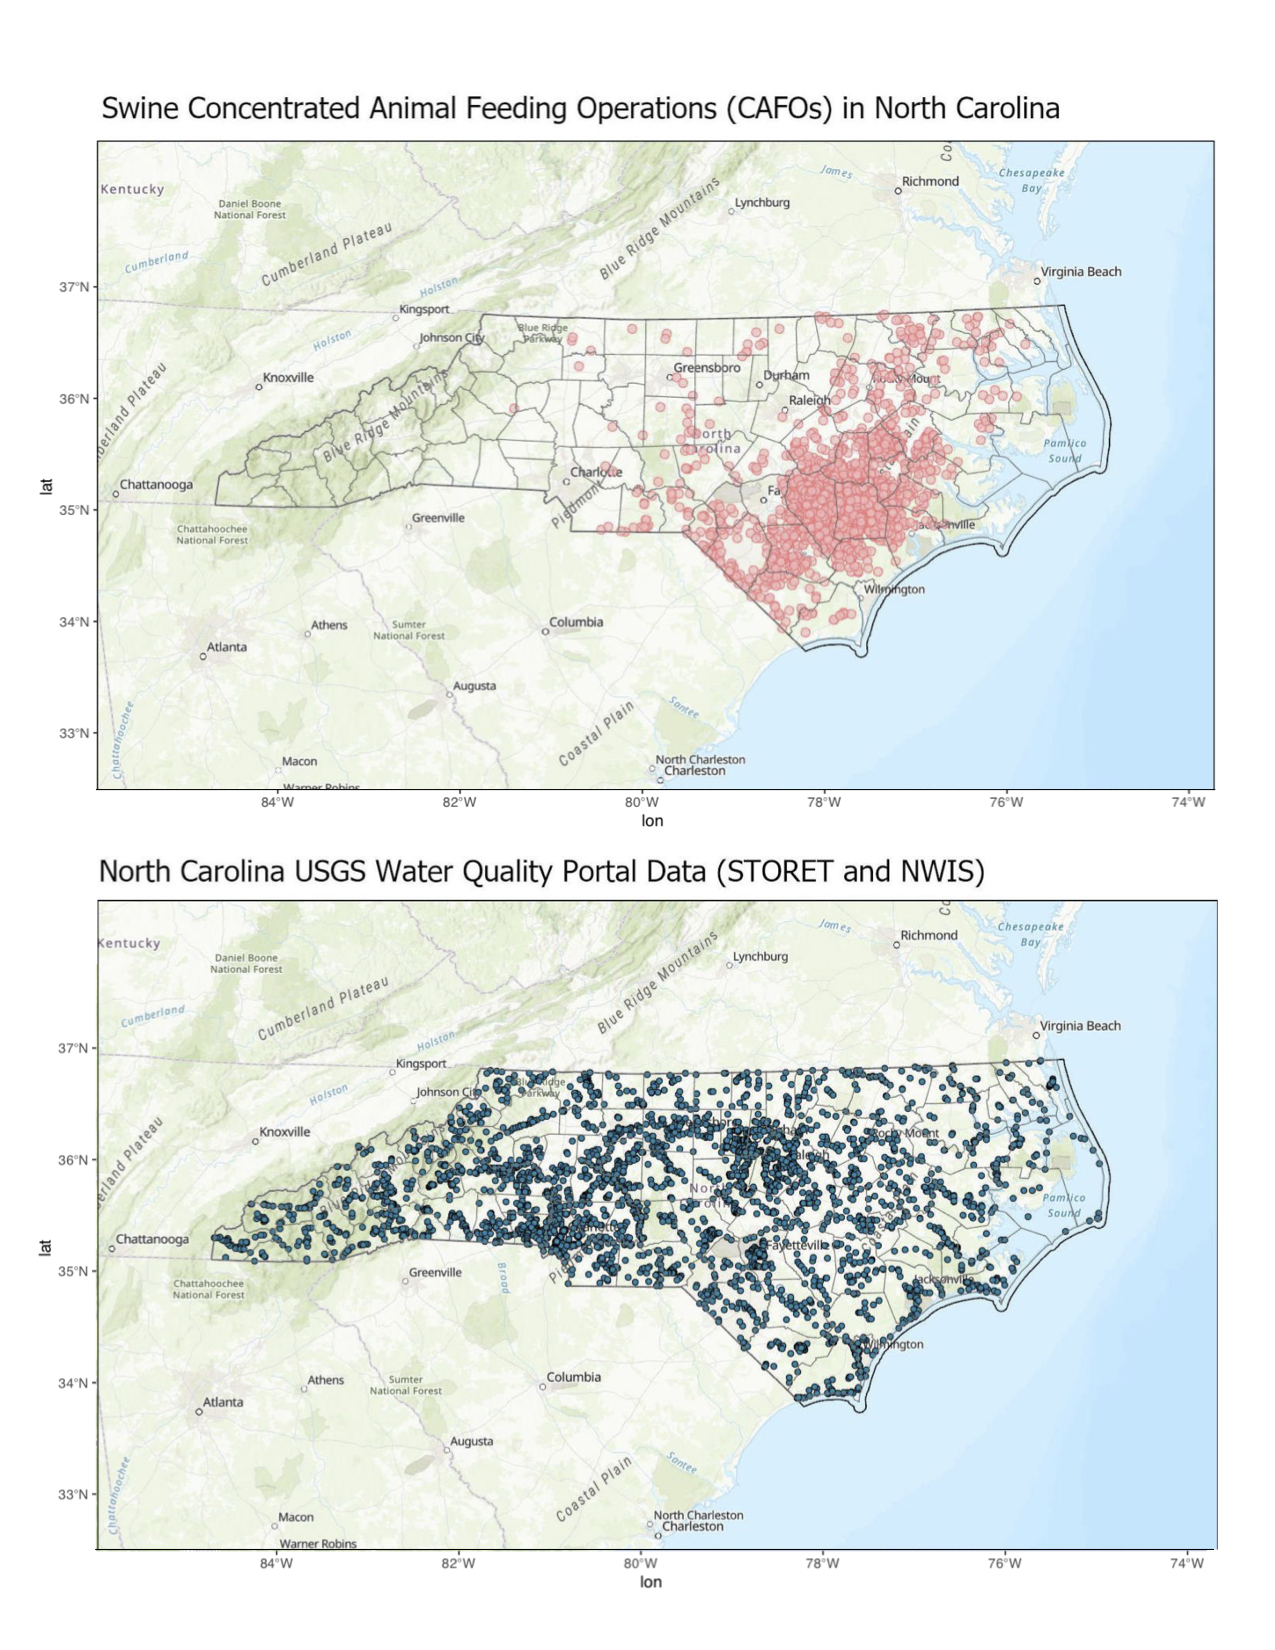
\includegraphics{swine_CAFO.png} \newpage

\#\#2.3 Data-Wrangling Process

The data from WQP was downloaded in two parts: a csv file of the site
information and a csv file of the microbiological sample results. These
sites and results datasheets have a common data field, ``monitoring
location ID'', that was used to join the two datasets together. The
initial downloaded dataset contained 73 columns in the raw dataset that
was then filtered to 25 columns in the processed dataset. Further
analysis for case studies wrangled the dataset into four columns.

\#\#2.4 Dataset Structure

The processed dataset contains 25 columns, which are described in Table
2. Further analysis for case studies wrangled the dataset into five
columns shown in Table 3. A breakdown of North Carolina counties by
their associated USGS code is provided in Table 4.

\newpage

\hypertarget{exploratory-data-analysis}{%
\subsubsection{3. Exploratory Data
Analysis}\label{exploratory-data-analysis}}

The raw microbiological data collected contained superfluous information
that needed to be removed to only contain information pertinent to the
analysis (Table 2). Fecal coliform samples were collected from 4,618
water quality monitoring stations observed across 98 counties in North
Carolina. Fecal coliform was near or above the EPA recommend
concentrations across 98 sites in surface waters (Figure 2).
Concentrations ranged from 0-31,000,000 cfu/100 ml, and upon further
exploration, 95 counties recorded samples exceeding the EPA recommend
200 cfu/100 ml concentration. The remaining three North Carolina
counites: Gates, Pamlico, and Dare, all had concentrations well below
the recommend limit.

\#\#3.1 Exploration of Fecal Coliform Concentrations in relation to N.C.
County Data

Visual data exploration of the recorded samples of fecal coliform are
illustrated in Figures 2 through Figure 7. This initial exploration of
data provided insights into potential correlations between counties and
fecal coliform concentrations, as well as how concentrations changed
over the past 48 years.
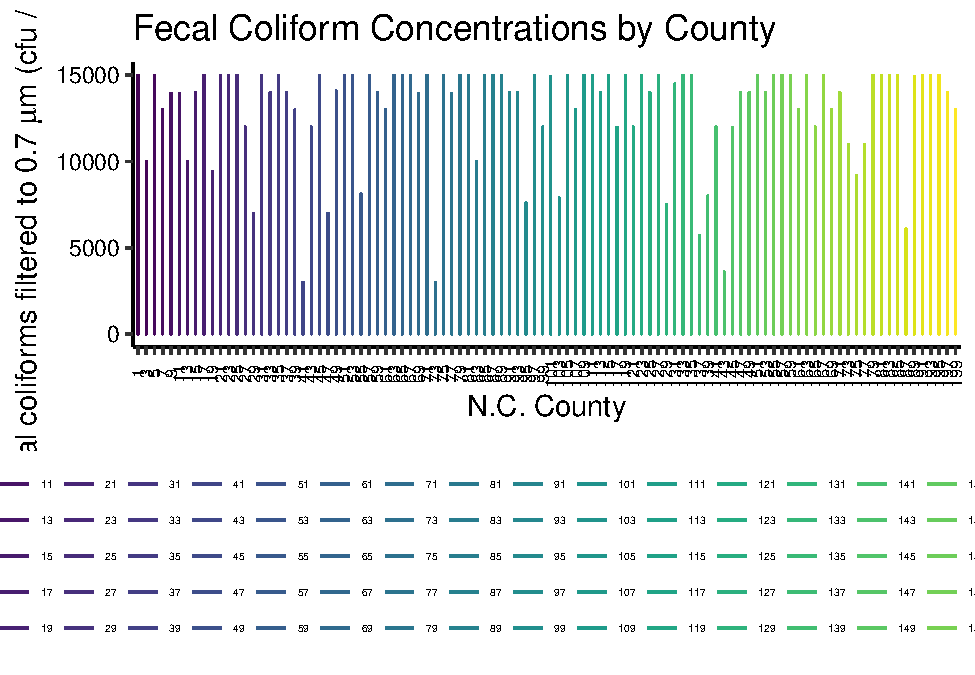
\includegraphics{Edmondson_ENV872_Project_files/figure-latex/unnamed-chunk-1-1.pdf}

\begin{figure}
\centering
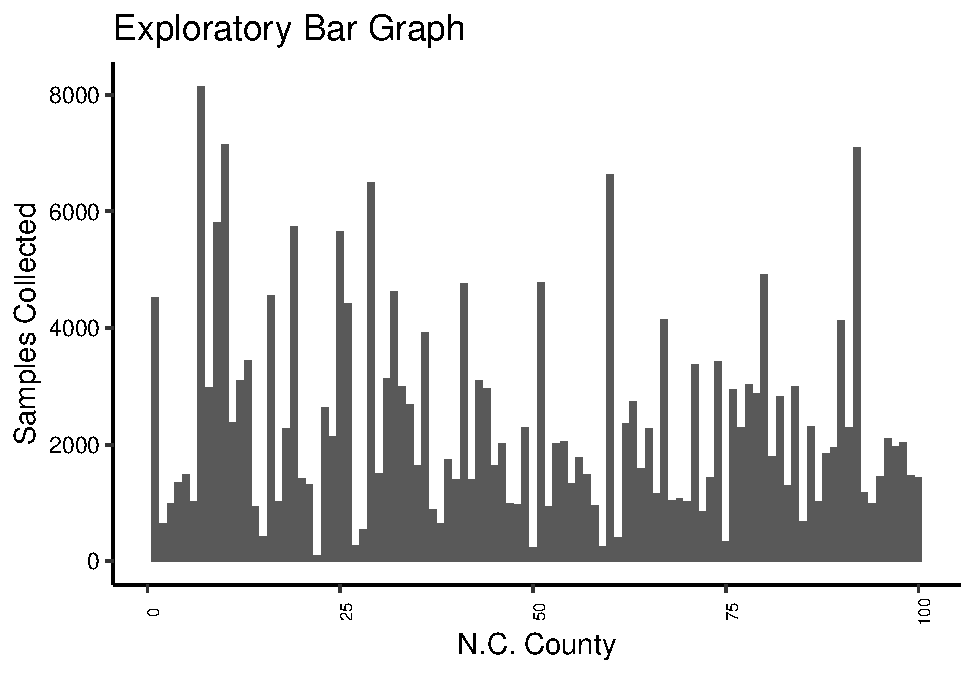
\includegraphics{Edmondson_ENV872_Project_files/figure-latex/unnamed-chunk-3-1.pdf}
\caption{Figure 4: Recorded Fecal Coliform Samples Per County}
\end{figure}

\begin{figure}
\centering
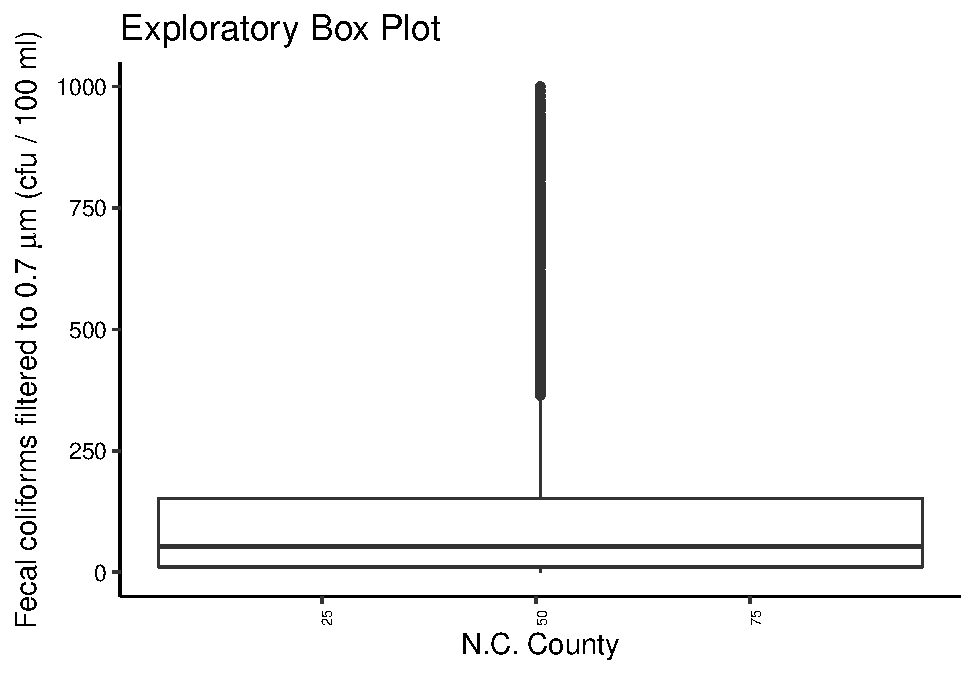
\includegraphics{Edmondson_ENV872_Project_files/figure-latex/unnamed-chunk-4-1.pdf}
\caption{Figure 5. Box Plot of Fecal Coliform Data across N.C. Counties}
\end{figure}

\begin{figure}
\centering
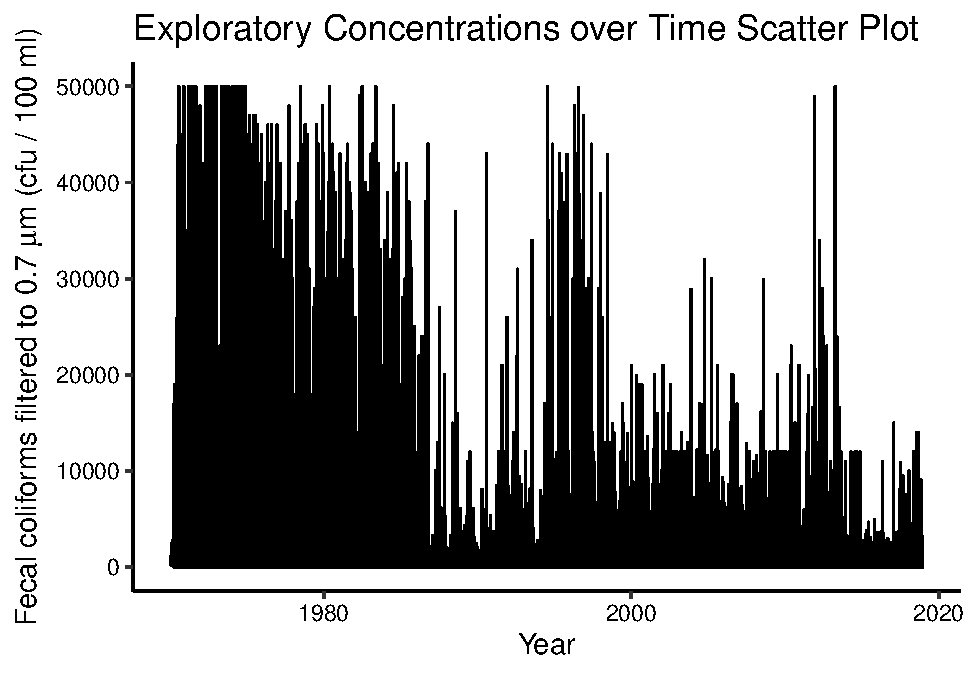
\includegraphics{Edmondson_ENV872_Project_files/figure-latex/unnamed-chunk-6-1.pdf}
\caption{Figure 7. Recorded Fecal Coliform Concentrations from
1970-2018}
\end{figure}

\#\#3.2 Exploration of the Proposed Six Case Study Counties

From the exploratory analysis above, six counties with the highest
concentrations of swine concentrated animal feeding operations had
notable exceedances in fecal coliform concentrations in surface waters
(Table 5). Additional exploratory analysis was conducted to determine
emerging trends in the relationship between fecal coliform
concentrations across years and across seasons. Visual data exploration
of the recorded samples of fecal coliform are illustrated in Figures 9
through Figure 26. A map of the extent of the case study area is
provided in Figure 8.

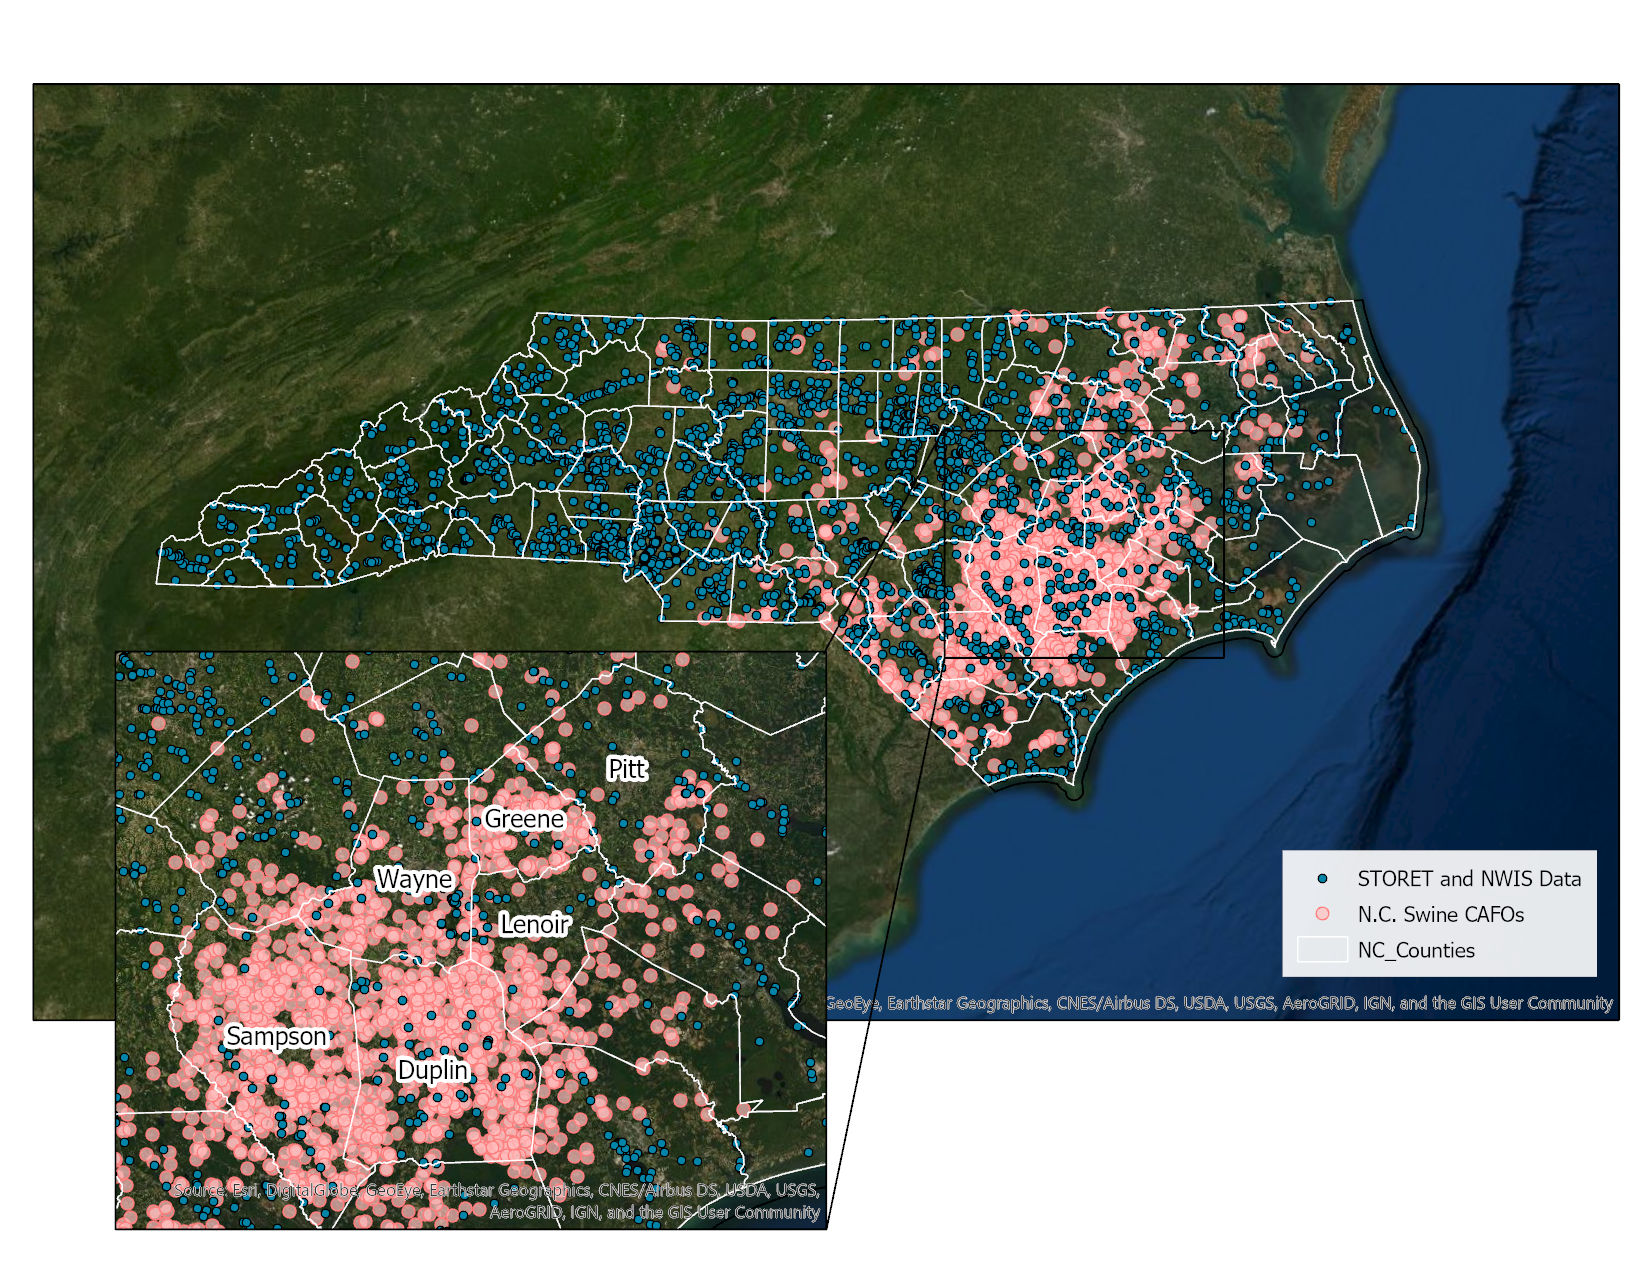
\includegraphics{extent_map.png}
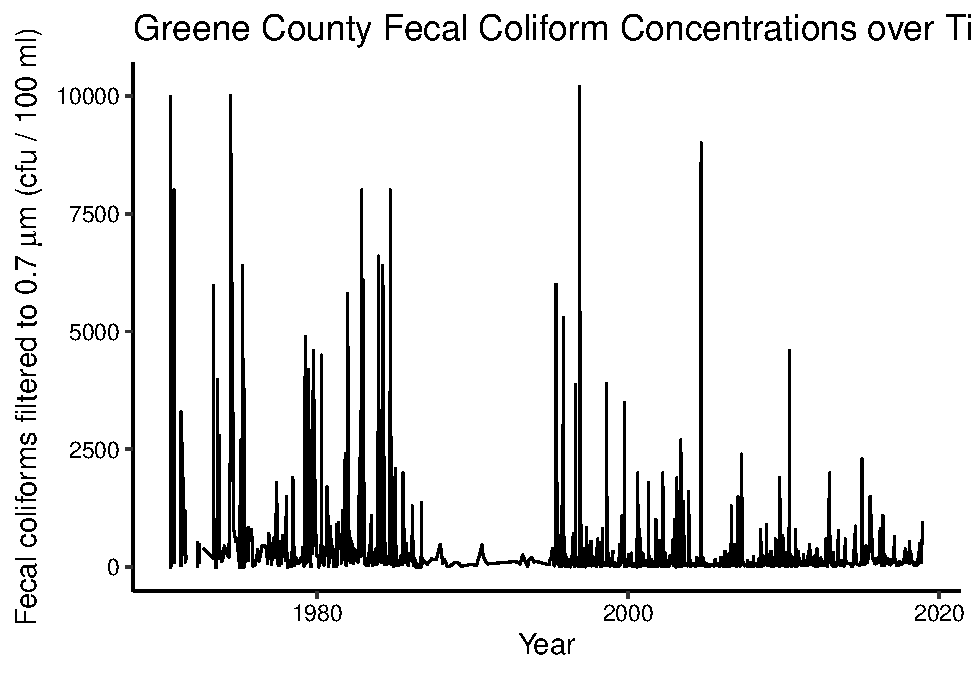
\includegraphics{Edmondson_ENV872_Project_files/figure-latex/unnamed-chunk-7-1.pdf}

\begin{figure}
\centering
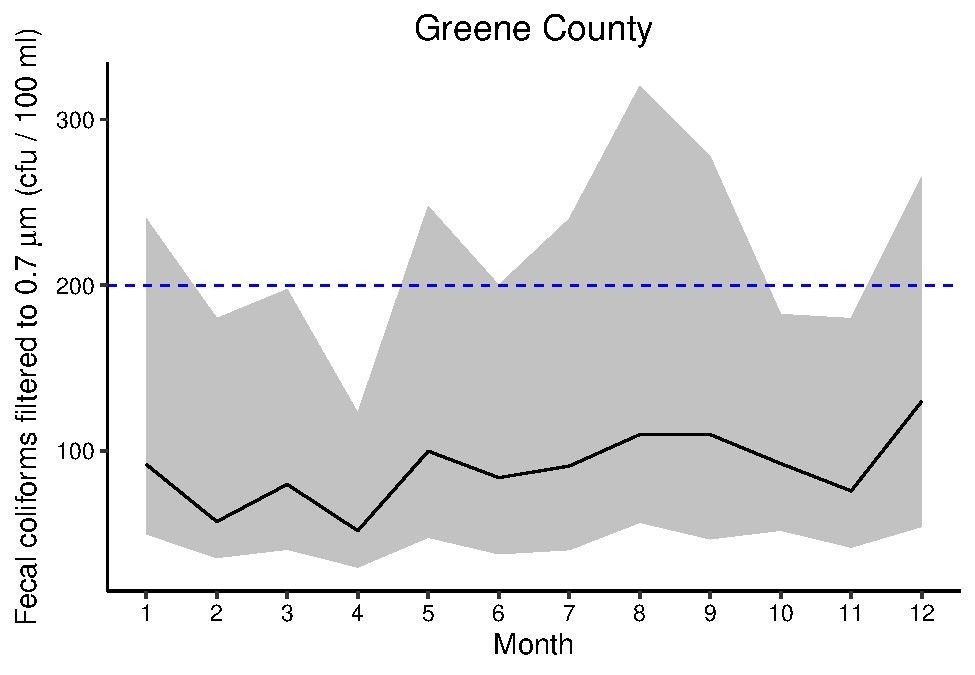
\includegraphics{Edmondson_ENV872_Project_files/figure-latex/unnamed-chunk-9-1.pdf}
\caption{Figure 10. Exploratory plot of recorded seasonal fecal coliform
concentations in Greene County, N.C.}
\end{figure}

\begin{figure}
\centering
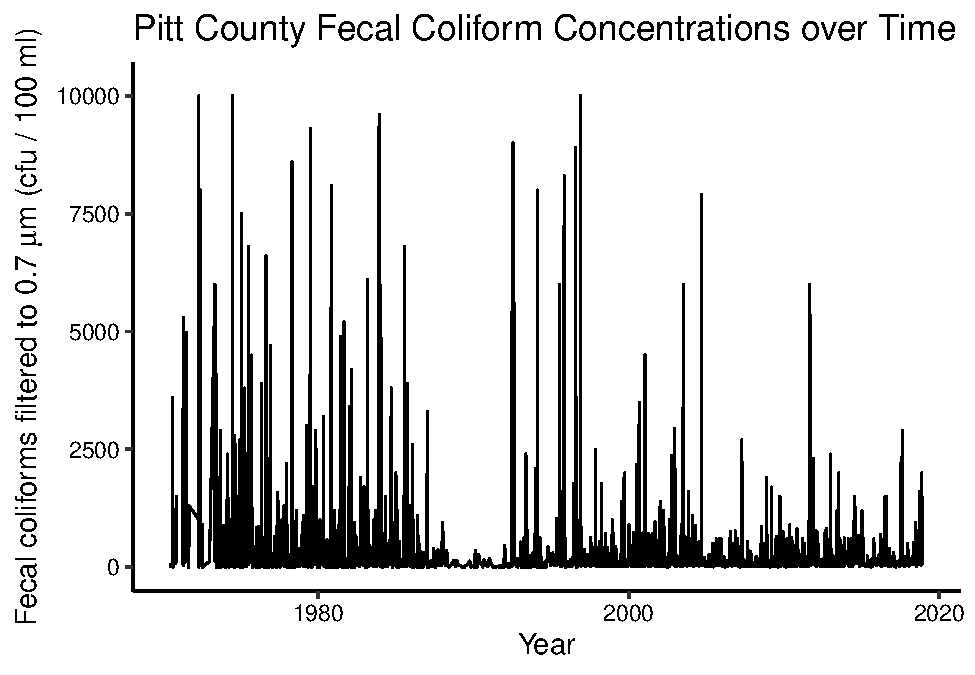
\includegraphics{Edmondson_ENV872_Project_files/figure-latex/unnamed-chunk-10-1.pdf}
\caption{Figure 11. Exploratory plot of recorded fecal coliform
concentations in Pitt County, N.C.}
\end{figure}

\begin{figure}
\centering
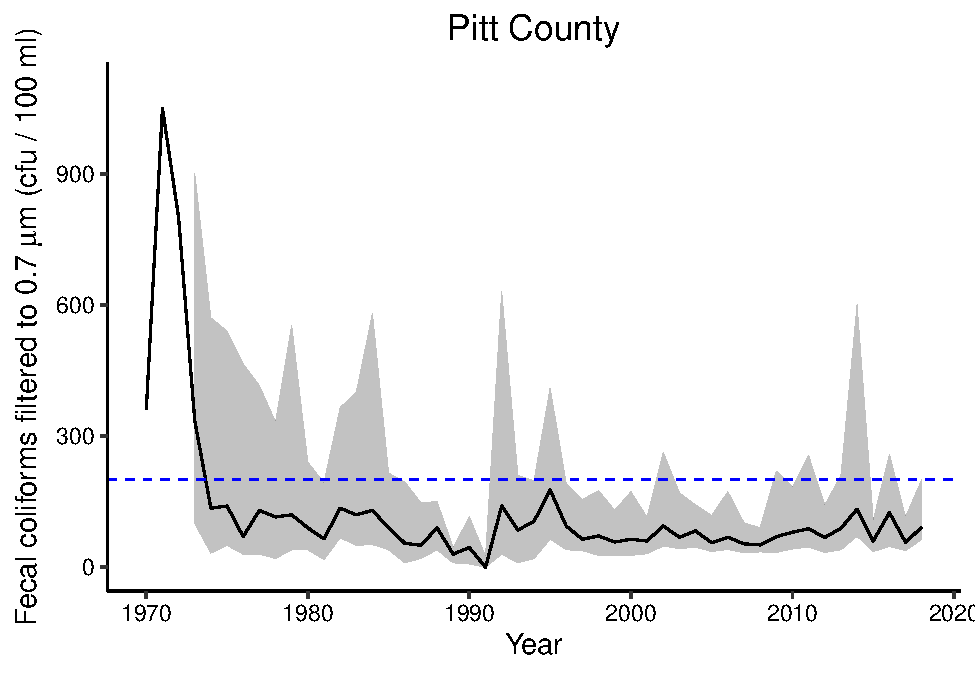
\includegraphics{Edmondson_ENV872_Project_files/figure-latex/unnamed-chunk-11-1.pdf}
\caption{Figure 12. Exploratory plot of recorded fecal coliform
concentations in Pitt County, N.C. from 1970- 2018}
\end{figure}

\begin{figure}
\centering
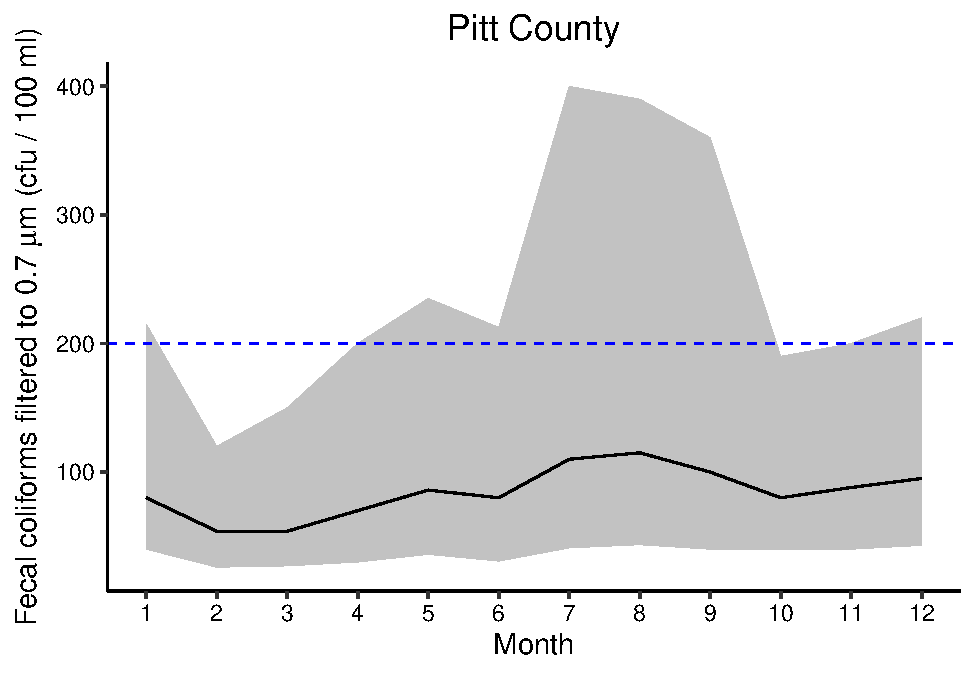
\includegraphics{Edmondson_ENV872_Project_files/figure-latex/unnamed-chunk-12-1.pdf}
\caption{Figure 13. Exploratory plot of recorded seasonal fecal coliform
concentations in Pitt County, N.C}
\end{figure}

\begin{figure}
\centering
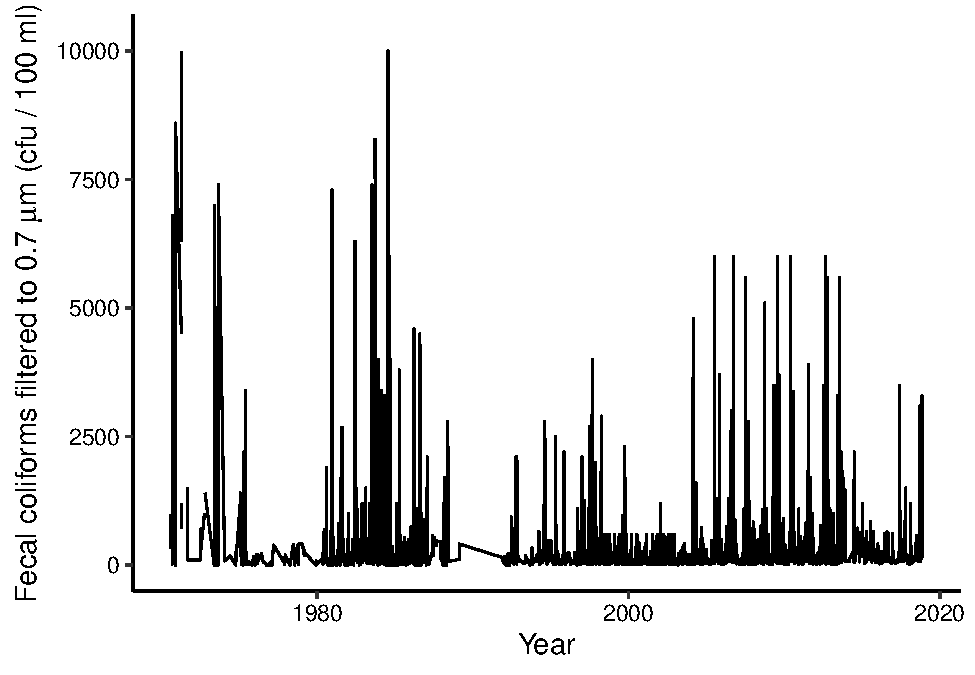
\includegraphics{Edmondson_ENV872_Project_files/figure-latex/unnamed-chunk-13-1.pdf}
\caption{Figure 14. Exploratory plot of recorded fecal coliform
concentations in Duplin County, N.C.}
\end{figure}

\begin{figure}
\centering
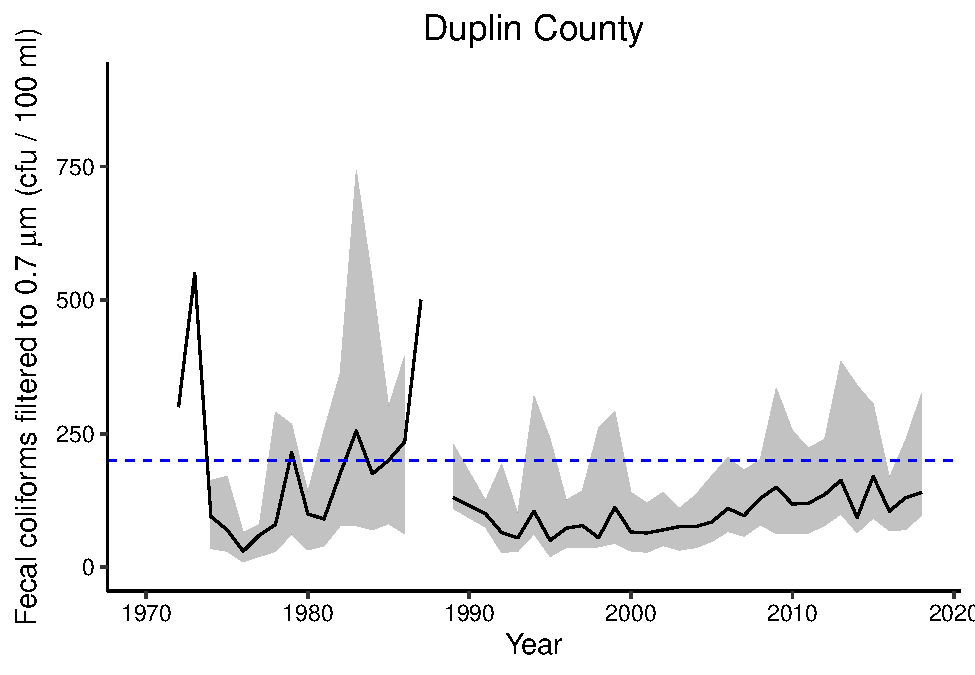
\includegraphics{Edmondson_ENV872_Project_files/figure-latex/unnamed-chunk-14-1.pdf}
\caption{Figure 15. Exploratory plot of recorded seasonal fecal coliform
concentations in Duplin County, N.C}
\end{figure}

\begin{figure}
\centering
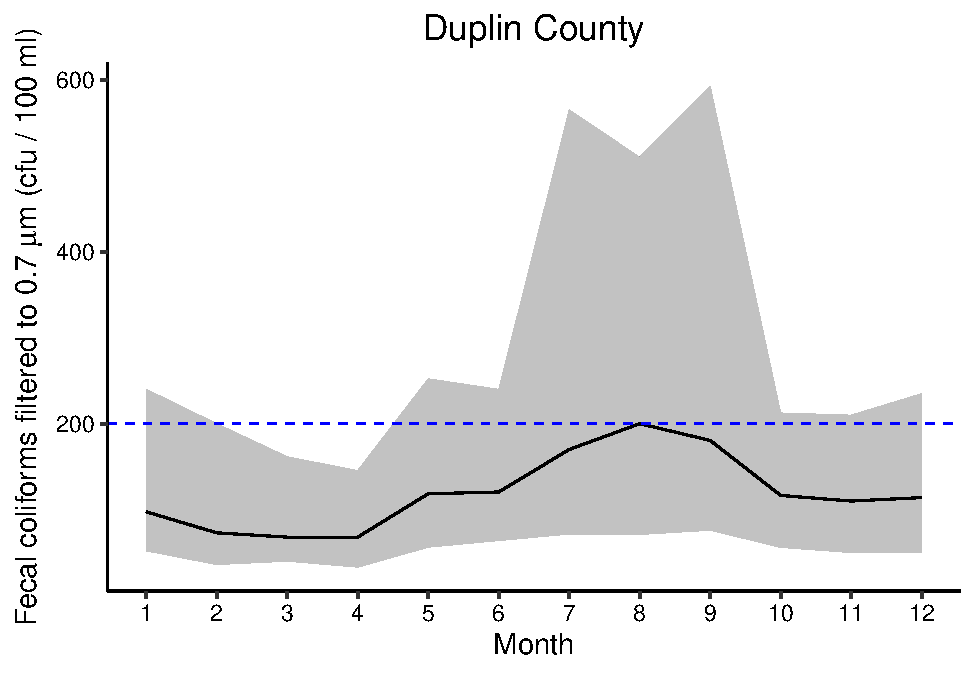
\includegraphics{Edmondson_ENV872_Project_files/figure-latex/unnamed-chunk-15-1.pdf}
\caption{Figure 16. Exploratory plot of recorded seasonal fecal coliform
concentations in Duplin County, N.C}
\end{figure}

\begin{figure}
\centering
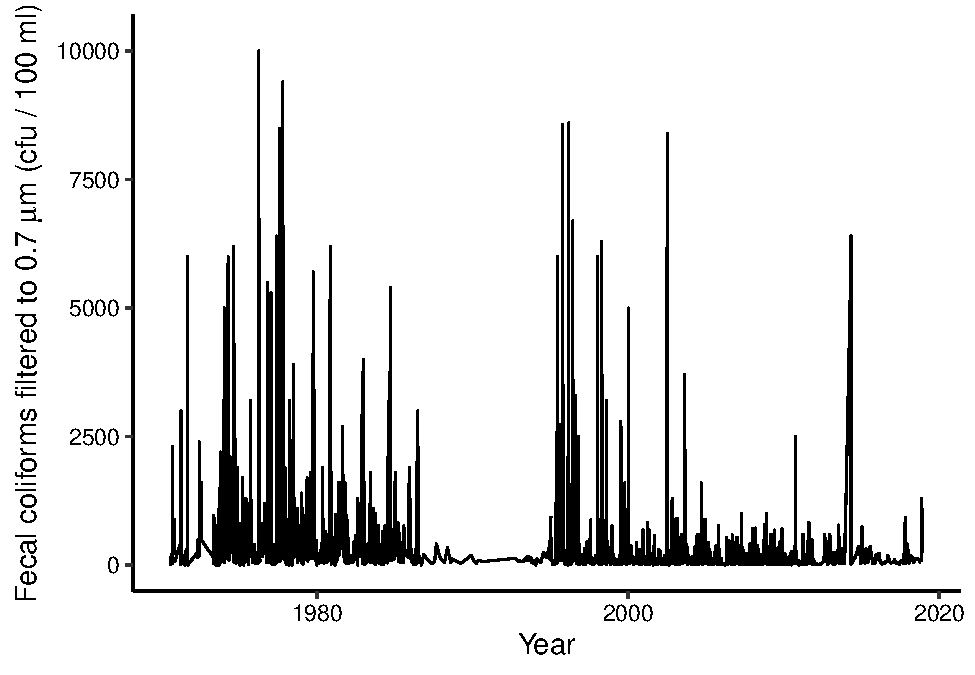
\includegraphics{Edmondson_ENV872_Project_files/figure-latex/unnamed-chunk-16-1.pdf}
\caption{Figure 17. Exploratory plot of recorded seasonal fecal coliform
concentations in Lenoir County, N.C}
\end{figure}

\begin{figure}
\centering
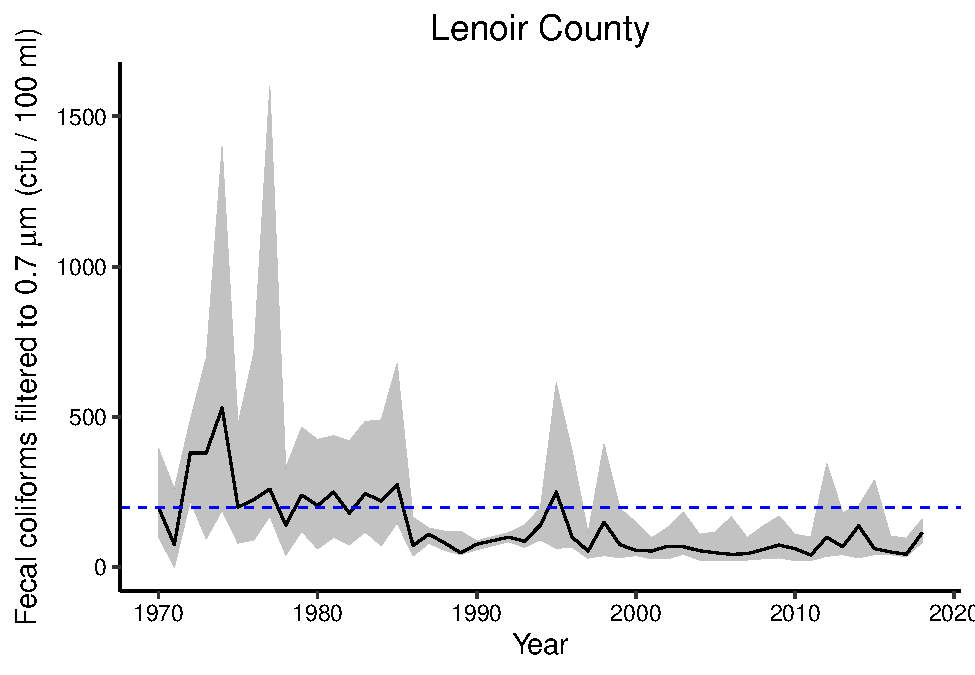
\includegraphics{Edmondson_ENV872_Project_files/figure-latex/unnamed-chunk-17-1.pdf}
\caption{Figure 18. Exploratory plot of recorded fecal coliform
concentations in Lenoir County, N.C. from 1970- 2018}
\end{figure}

\begin{figure}
\centering
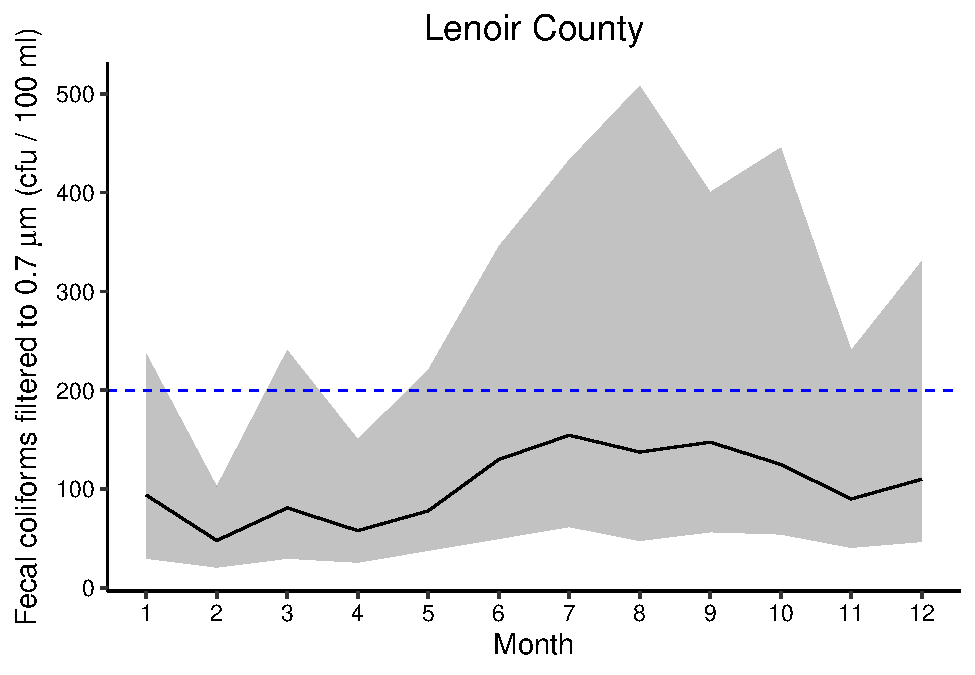
\includegraphics{Edmondson_ENV872_Project_files/figure-latex/unnamed-chunk-18-1.pdf}
\caption{Figure 19. Exploratory plot of recorded seasonal fecal coliform
concentations in Lenoir County, N.C}
\end{figure}

\begin{figure}
\centering
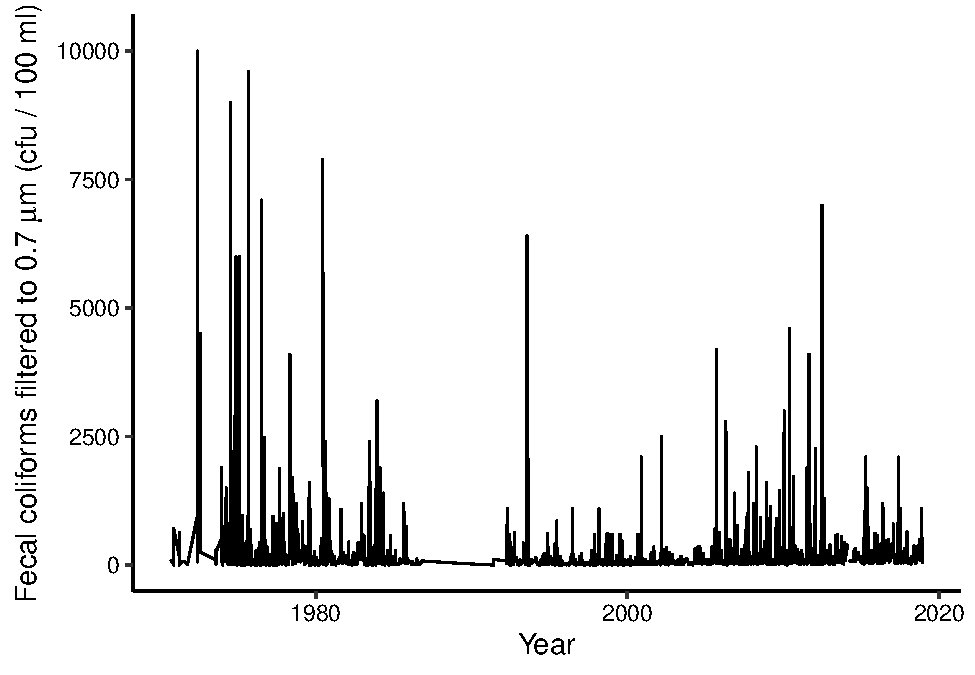
\includegraphics{Edmondson_ENV872_Project_files/figure-latex/unnamed-chunk-19-1.pdf}
\caption{Figure 20. Exploratory plot of recorded fecal coliform
concentations in Sampson County, N.C.}
\end{figure}

\begin{figure}
\centering
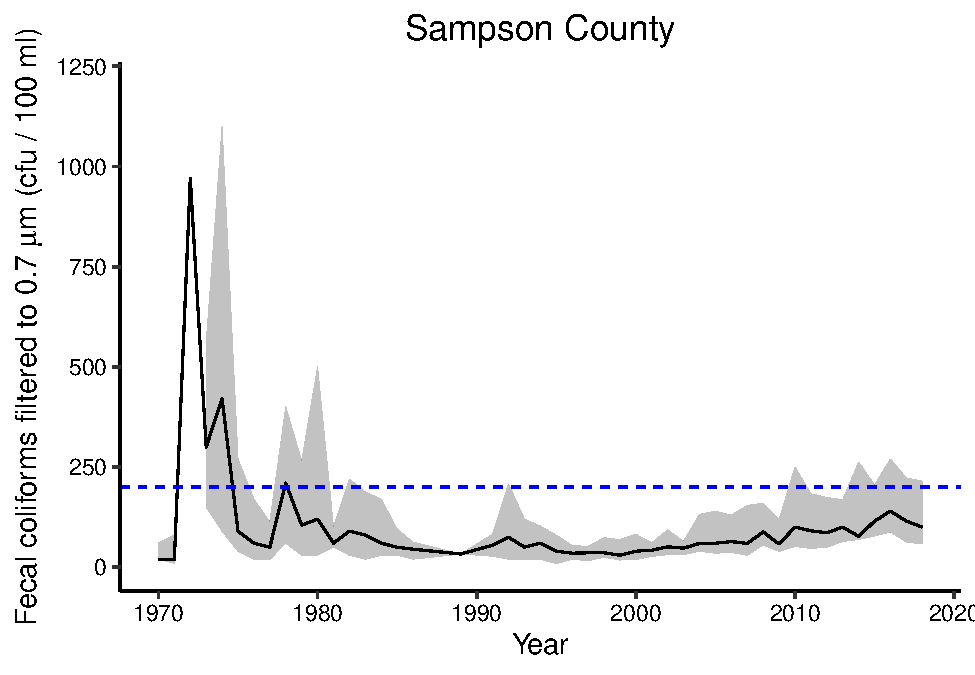
\includegraphics{Edmondson_ENV872_Project_files/figure-latex/unnamed-chunk-20-1.pdf}
\caption{Figure 21. Exploratory plot of recorded fecal coliform
concentations in Sampson County, N.C. from 1970- 2018}
\end{figure}

\begin{figure}
\centering
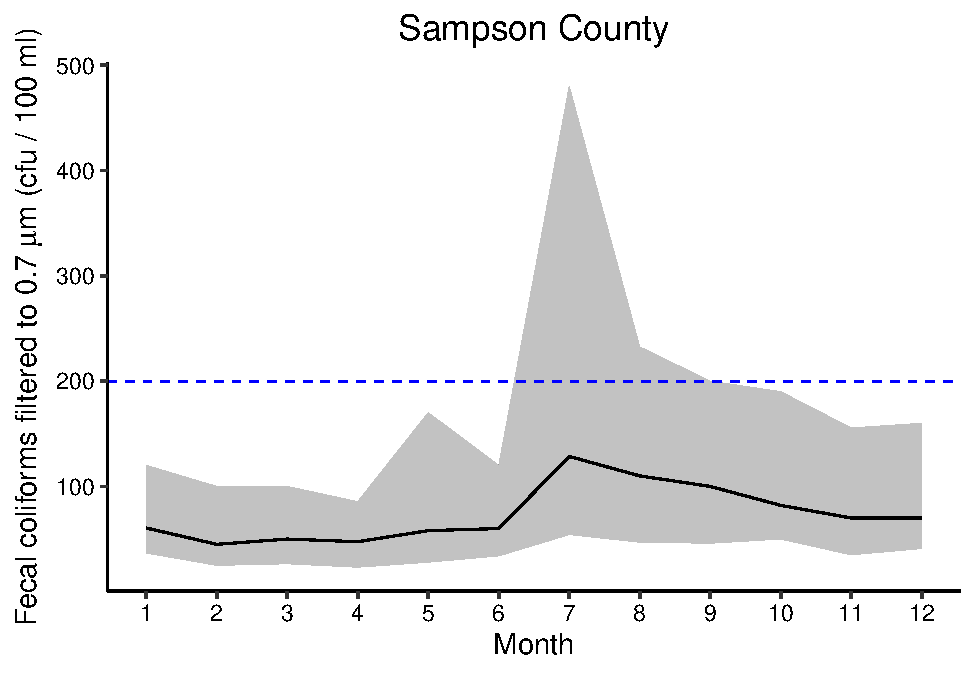
\includegraphics{Edmondson_ENV872_Project_files/figure-latex/unnamed-chunk-21-1.pdf}
\caption{Figure 22. Exploratory plot of recorded seasonal fecal coliform
concentations in Sampson County, N.C}
\end{figure}

\begin{figure}
\centering
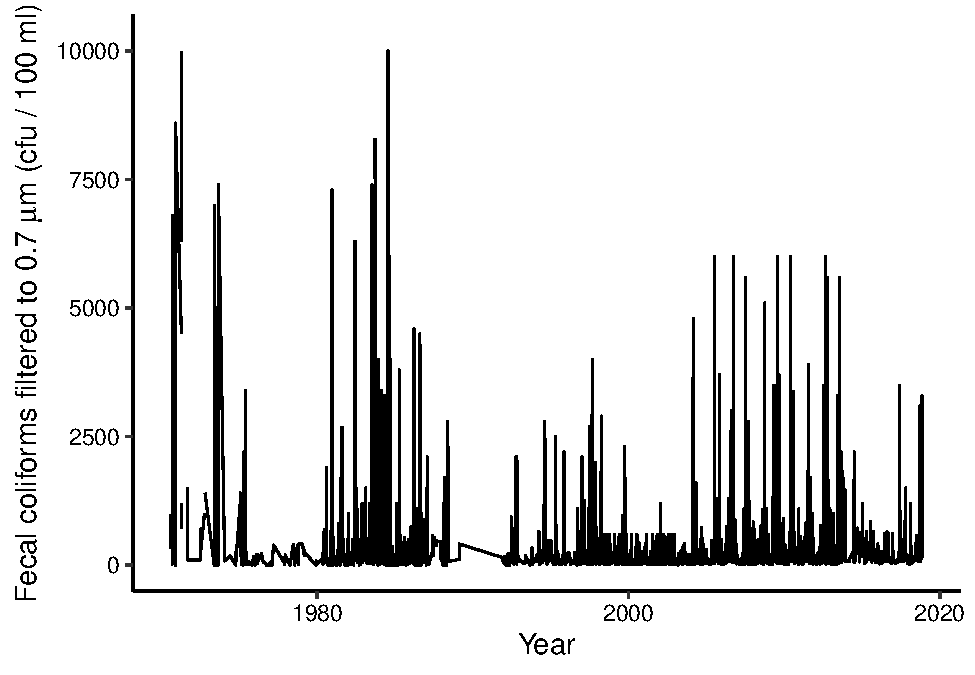
\includegraphics{Edmondson_ENV872_Project_files/figure-latex/unnamed-chunk-22-1.pdf}
\caption{Figure 23. Exploratory plot of recorded fecal coliform
concentations in Wayne County, N.C.}
\end{figure}

\begin{figure}
\centering
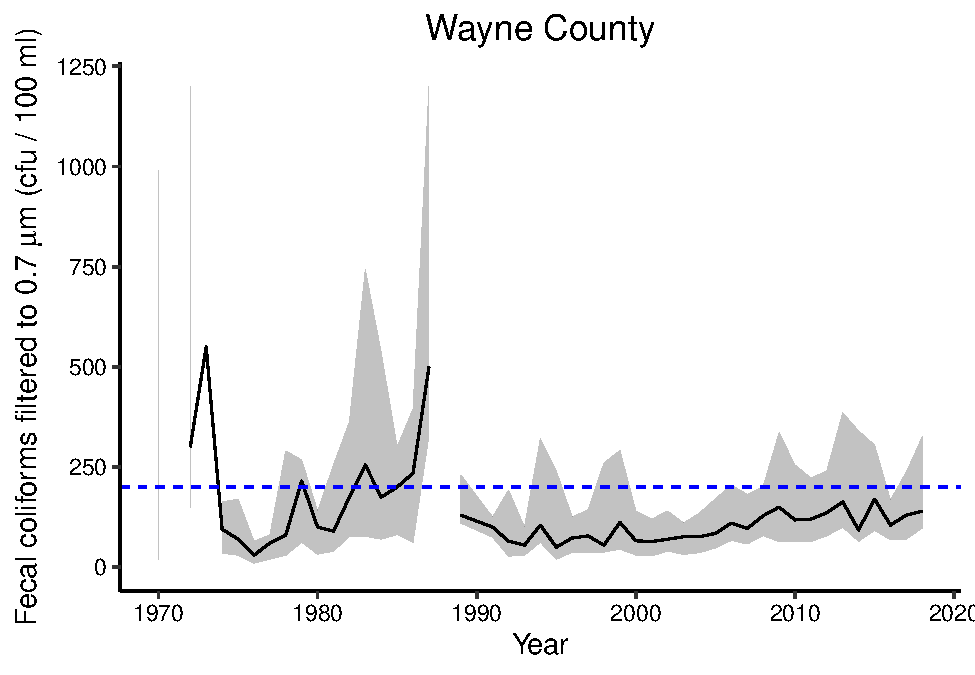
\includegraphics{Edmondson_ENV872_Project_files/figure-latex/unnamed-chunk-23-1.pdf}
\caption{Figure 24. Exploratory plot of recorded fecal coliform
concentations in Wayne County, N.C. from 1970- 2018}
\end{figure}

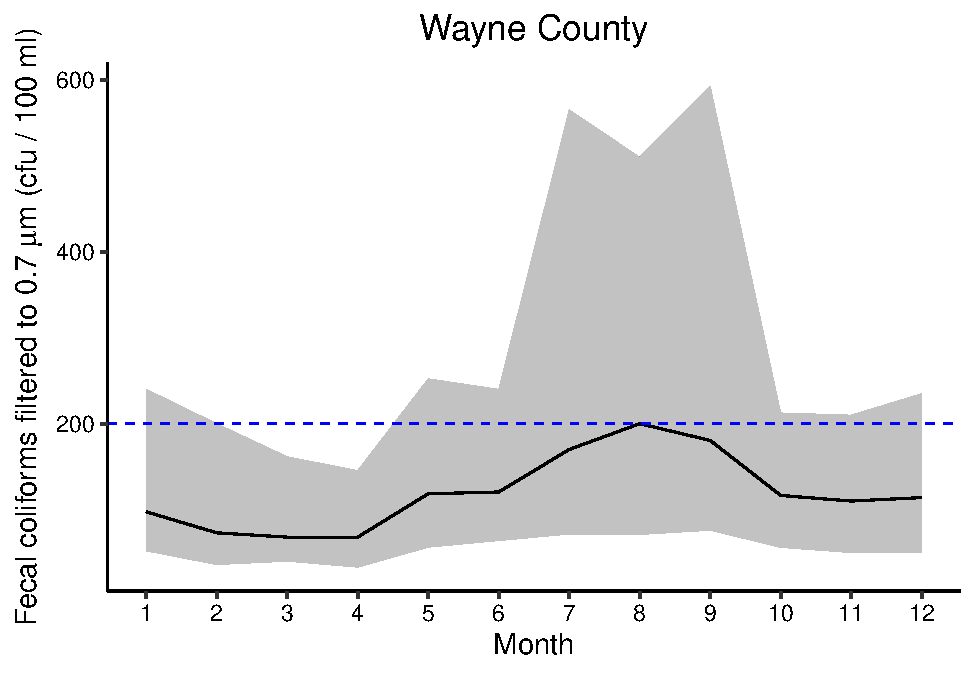
\includegraphics{Edmondson_ENV872_Project_files/figure-latex/unnamed-chunk-24-1.pdf}
\newpage

\hypertarget{analysis}{%
\subsubsection{4. Analysis}\label{analysis}}

Generalized linear models (GLMs) were used throughout this analysis to
determine if there is a linear combination of the effects of categorial
or continuous explanatory variables. The inclusion of these models
allows a fit to the main effects of both categorical and continuous
explanatory variables as well as their interactions. The GLM is based on
the assumption that the data residuals approximate a normal distribution
(or a linearly transformed normal distribution). For tests that analyze
categorical explanatory variables, the assumption is that the variance
in the response variable is equal among groups. It is important to note
that environmental data often violate the assumptions of normality and
equal variance, and will often proceed with a GLM even if these
assumptions are violated.

\#\#4.1 One-sample T-Test

The first statistical analysis will test the null hypothesis that the
mean of fecal coliform concentrations in North Carolina are below the
regulatory standard of 200 cfu/100ml. The first assumption of the normal
distribution is evaluated. The processed dataset was tested for
normality using the Shapiro-Wilks normality test. This test determined
that for all 100 N.C. counties fecal coliform concentrations are
significantly different from a normal distribution, and to reject the
null hypothesis (Shapiro-Wilks normality test, W = 0.30-0.07 , p-value
\textless{} 0.0001). The p-value for the Shapiro-Wilk test is
\textless{}0.001 suggesting the data is not normally distributed. An
additional normalcy tests, qqnorm and qqline, were applied to the
dataset to determine the distribution (Figure \_\_\_). The normal Q-Q
plot suggests that the data is approximately normal with a few outliers
in the 4th quartile.

\begin{figure}
\centering
\includegraphics{Edmondson_ENV872_Project_files/figure-latex/unnamed-chunk-25-1.pdf}
\caption{Figure 26. QQ plot results}
\end{figure}

The Bartlett test of homogeneity as used test to check for equal
variance among the dataset. The null hypotheses is that the variance is
the same for all product lines. Since the test statistic is greater than
the critical value for the chi-square and the p-value is less than
0.001, there is a significant difference in the variances (Bartlett's
K-squared = 977974, df =99, p-value \textless{}0.001). This means that
there is evidence to suggest that the variance in fecal coliform
concentrations is different among North Carolina counties. \newpage

\#\#4.2 One-Way ANOVA

A one-way ANOVA test was preformed to determine if there was a
significant correlation between N.C. counties and fecal coliform
concentrations. This test requires a second assumption to be complied,
which is that the variance of the groups is equal across groups.
Understanding that the data set is not perfectly normal, to test for the
homogeneity of variance across groups a Bartlett test was used as well
as a Fligner-Killeen test.

The Fligner-Killeen test of homogeneity of variances says that the
variance across groups is not homogeneous, but with a p-value close to
0.05 (med chi-squared = 44111, p-value = 0.001 \textless{} 0.05). For
this reason, for testing if there are significant differences between
the fecal coliform concentrations among N.C. counties, it is used a
One-way ANOVA test and a Non-parametric equivalent of ANOVA, the
Kruskal-Wallis Test.

A one-way ANOVA test revealed that there is significant correlation
between N.C. counties and fecal coliform concentrations (p-value
\textless{} 0.001). The linear model reveled that eight N.C. counties
are significantly different (multiple R-squared: 0.00244, F-statistic:
5.411, p-value \textless{}0.01). The eight counties that are
significantly different are Anson, Forsyth, Gaston, Martin,
Mecklendburg, Rockingham, Richmond, Wayne. Both Davidson and Orange
county had a slight correlation of fecal coliform with a p-value of 0.1.
This analysis also revealed that there was no clear significant impact
on exceeding fecal coliform concentrations in proximity to swine CAFOs.
\newpage

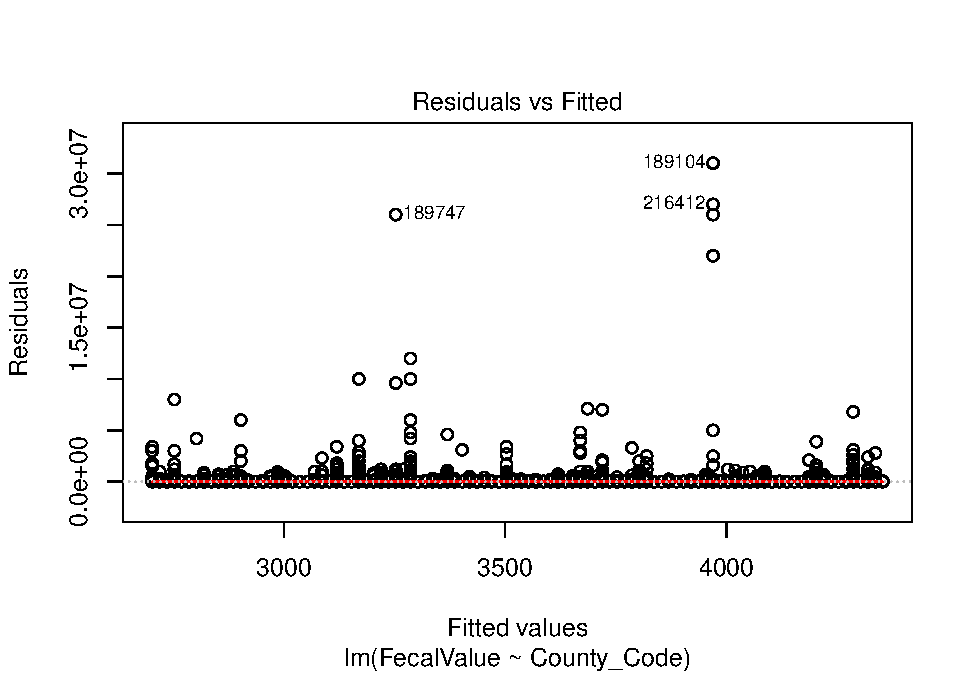
\includegraphics{Edmondson_ENV872_Project_files/figure-latex/unnamed-chunk-26-1.pdf}
\includegraphics{Edmondson_ENV872_Project_files/figure-latex/unnamed-chunk-26-2.pdf}
\includegraphics{Edmondson_ENV872_Project_files/figure-latex/unnamed-chunk-26-3.pdf}
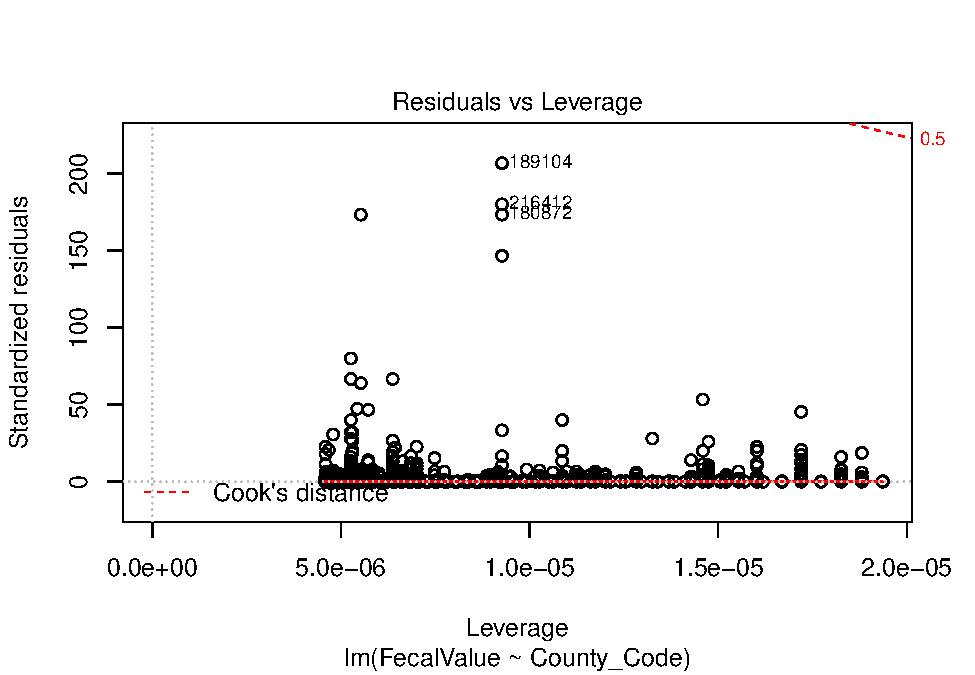
\includegraphics{Edmondson_ENV872_Project_files/figure-latex/unnamed-chunk-26-4.pdf}

To analyze which counties are different, post hoc tests: a Tukey
multiple comparisons of means test for ANOVA and a Dunn's test for
Kruskal-Wallis were used. According to both tests, there is a
significant difference between the fecal coliform concentrations for the
different counties in N.C. (ANOVA; F = 5.41, df = 99, p \textless{}
2.2e-16) (Kruskal-Wallis chi-squared = 33796, df = 99, p-value
\textless{} 2.2e-16).
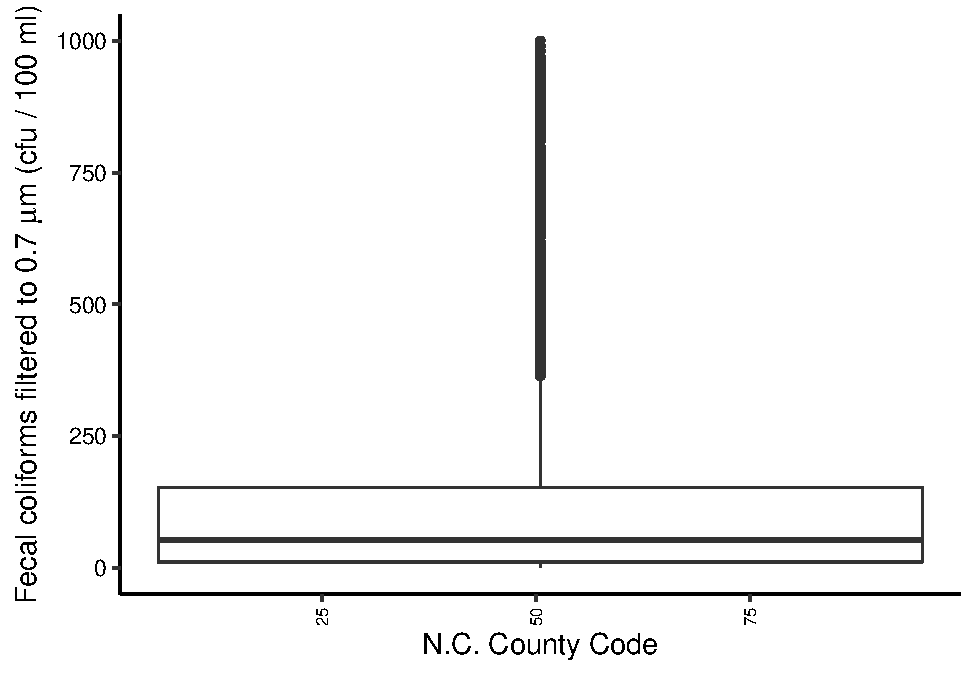
\includegraphics{Edmondson_ENV872_Project_files/figure-latex/unnamed-chunk-27-1.pdf}

\#\#4.3 Time Series

Case studies were conducted for six counties in North Carolina that have
the highest ratio of permitted swine CAFOs in the state. Time series
graphs were created to assess emerging trends in fecal coliform
concentrations across season and across the 48 year time frame (Figure
30).

\begin{figure}
\centering
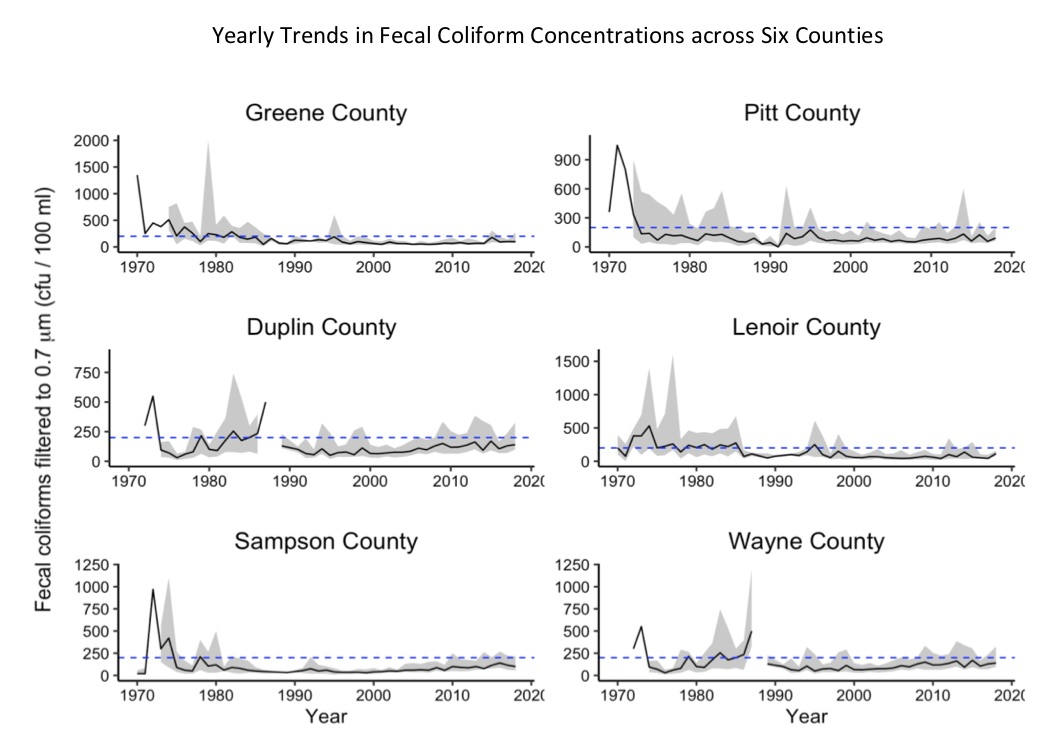
\includegraphics{Yearly_trends.png}
\caption{Figure 30. Yearly trends in Fecal Coliform Concentrations}
\end{figure}

\begin{figure}
\centering
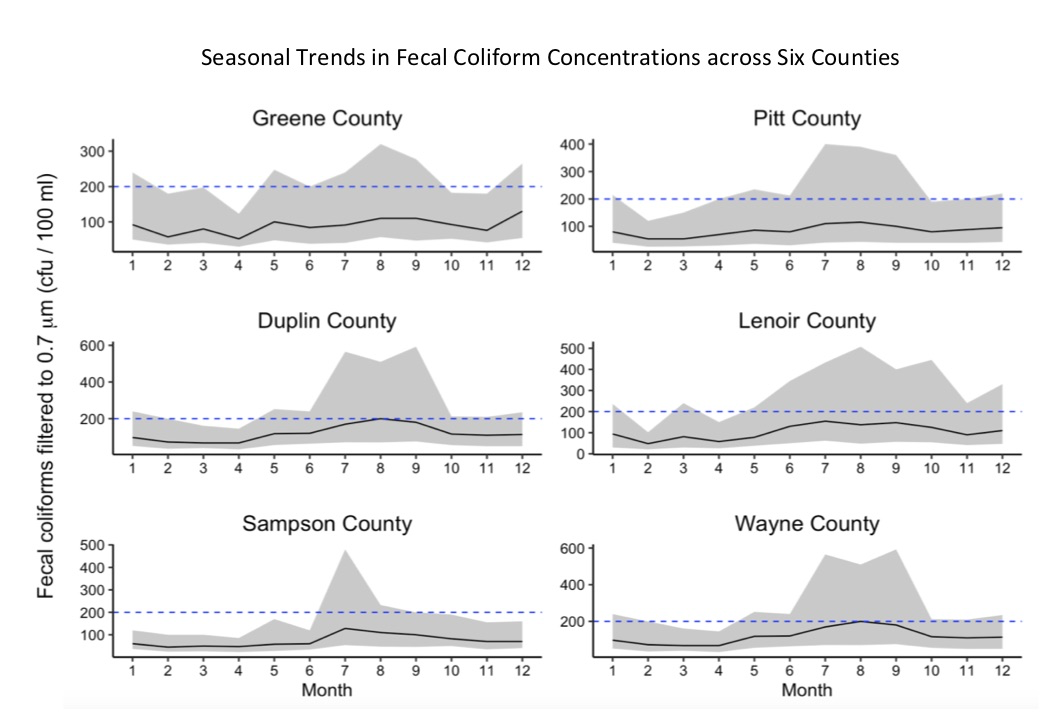
\includegraphics{Seasonal_trends.png}
\caption{Figure 31. Seasonal trends in Fecal Coliform Concentrations}
\end{figure}

A one-way ANOVA test was preformed to determine if there was a
significant correlation between a specific year or seasons in which
fecal coliform concentrations notably exceed EPA limits. The one-way
ANOVA test revealed that there is significant correlation between
seasons, specific years, and fecal coliform concentrations (p-value
\textless{} 0.001). The years that saw the highest concentrations of
fecal coliform across all six counites were from 1970 to 1984. It was
hypothesized that this time frame would see the highest concentrations
of fecal coliform because it was at a peak time for the industrial farm
industry, and regulations from the newly adopted Clean Water Act in 1972
were not yet implemented. There were also some unpredicted significant
yearly trends in two counties: Wayne county and Greene county. Wayne
county only had two years (1972-1972) were fecal coliform concentrations
were significantly high, and from 1973 on, concentrations remained
fairly low. In addition, Greene county saw a significant exceedance in
fecal coliform concentrations across all twelve months in 2009.

This analysis also revealed a significant correlation between seasons
and fecal coliform concentrations in surface waters. Across all six
counties, the month of July saw the highest exceedance in fecal coliform
concentrations (p-value \textless{}0.001). Additionally, the months of
August, May, and September had the second highest exceedance in fecal
coliform concentrations (p-value \textless{}0.01) among these six
counties studied. This concentration exceedance correlates with warmer
weather and water surface waters that aid in the growth of fecal
coliform bacteria. Additionally, this time frame also corresponds to
field application of waste management onto farms.

\newpage

\hypertarget{summary-and-conclusions}{%
\subsection{5. Summary and Conclusions}\label{summary-and-conclusions}}

This report focused on the concentrations of fecal coliform bacteria in
surface waters of North Carolina. The study explored which N.C. counties
have the highest recorded microbiological contaminates in surface
waters. Additionally, six case studies were conducted in counties that
have the most permitted swine CAFOs in North Carolina to determine if
there was a significant correlation between a specific year or seasons
in which fecal coliform concentrations notably exceed EPA limits. The
analysis preformed indicated that 95 counties in N.C. had a mean
concentration higher than the regulatory standard across multiple years.
Moreover, it was found that there was no clear significant impact on
exceeding fecal coliform concentrations in proximity to swine CAFOs.
This result, could be due to the fact that data was only considered for
counties in close proximity to known permitted swine CAFOs.

In the time series for each case study, it is clear that fecal coliform
concentrations were highest in the late 1970s until the 1980s. This
spike is attributed to the growing number of industrial farms in North
Carolina and that regulations from the newly adopted Clean Water Act in
1972 were not yet implemented. Futhermore, there appears to be an
increasing trend in fecal coliform concentrations within surface waters
starting in 2010 to the present date. This study also reveals that
across 48 years, there is a seasonal trend in peak fecal coliform
concentrations in surface waters. The month of July and the month of
August have the highest records of fecal coliform concentrations, and
peak seasons usually occur from May until October. The coincides with
warmer surface temperatures that can grow bacteria rapidly, as well as
spray-field waste application times.

North Carolina waters are a crucial to economy and livelihood of its
citizens. Variables such as seasons, years, locations, and contaminates
can be used to estimate the health of these waterways. The results of
this report can provide answers to regulators, managers, and key
stakeholders to improve environmental management and disease prevention.
This information can be used to improve water quality regulations in
N.C. and set a precedence for the state. \newpage

\end{document}
